\section{Results and Analysis}\label{sec:results}

\subsection{Feature Importance, and a Result We Do Not Bury}\label{sec:engine-finding}

Table~\ref{tab:topology-importance} reports each topology feature's XGBoost
gain importance~\cite{chen2016xgboost}, normalized within the full
topology-augmented model (\texttt{topology\_full} arm) for each of the four
datasets carrying a complete ablation run. Because these thirteen columns
sit alongside 15--21 ordinary tabular features in that model (BankSim: 21
ordinary + 13 topology = 34; IBM AML: 8 + 13 = 21; SAP Würzburg: 20 + 13 =
33; synth\_erp: 15 + 13 = 28), the rows below do not sum to $1$ within a
dataset — the remaining gain mass sits with the ordinary features, not shown
here. SAP Würzburg's split sizes in this table (120{,}411 / 40{,}137 /
40{,}139, partition-aware by \texttt{run\_id}) come from
\texttt{ablation.json} specifically; the paper's headline champion-model
table elsewhere draws on a very slightly different SAP split
(120{,}341 / 40{,}114 / 40{,}116) recorded in \texttt{final\_champions.json} — the
two pipelines' SAP preprocessing diverged by 70 rows in the training split
and 23 rows in each of validation and test, and
the two are never mixed within one reported number.

\begin{table}[t]
\centering
\caption{Topology feature gain importance (fraction of total gain in the
topology-augmented model), by dataset. Source:
\texttt{paper/data/ablation.json}, \texttt{topology\_importance}, single
seed, no confidence intervals.}
\label{tab:topology-importance}
\resizebox{\columnwidth}{!}{%
\begin{tabular}{lrrrr}
\toprule
\textbf{Feature} & \textbf{BankSim} & \textbf{IBM AML} & \textbf{SAP Würzburg} & \textbf{synth\_erp} \\
\midrule
\texttt{in\_cycle}           & 0.0000 & 0.0000 & 0.0000 & 0.0040 \\
\texttt{cycle\_length}       & 0.0000 & 0.0009 & 0.0000 & 0.0029 \\
\texttt{in\_cycle\_ge3}      & 0.0000 & 0.0000 & 0.0000 & 0.0044 \\
\texttt{cycle\_amount\_ratio}& 0.0000 & 0.0008 & 0.0000 & 0.0090 \\
\texttt{cycle\_time\_span}   & 0.0000 & 0.0001 & 0.0000 & 0.0072 \\
\midrule
\texttt{fan\_in}             & 0.0908 & 0.0003 & 0.1791 & 0.0241 \\
\texttt{fan\_out}            & 0.0062 & 0.0010 & 0.0136 & 0.0189 \\
\texttt{dest\_in\_degree}    & 0.5199 & 0.0003 & 0.0682 & 0.0230 \\
\texttt{src\_out\_degree}    & 0.0062 & 0.0007 & 0.0089 & 0.0786 \\
\midrule
\texttt{lap\_in\_recur}      & 0.0052 & 0.0006 & 0.0319 & 0.0130 \\
\texttt{lap\_in\_payers}     & 0.0048 & 0.0006 & 0.0199 & 0.0103 \\
\texttt{lap\_out\_recur}     & 0.0066 & 0.5397 & 0.0416 & 0.0041 \\
\texttt{lap\_out\_payees}    & 0.0079 & 0.4200 & 0.0000 & 0.0036 \\
\bottomrule
\end{tabular}%
}
\end{table}

%% FIGURE TODO: grouped bar chart, one panel per dataset (BankSim, IBM AML,
%% SAP Würzburg, synth_erp), bars = gain importance for the 13 topology
%% features colour-coded by group (cycle / degree-fan / lapping), y-axis
%% shared across panels to make visually obvious that the 5 cycle-feature
%% bars are flat at zero in 3 of the 4 panels and barely visible in the 4th.
\begin{figure}[t]
\centering
% \includegraphics[width=\columnwidth]{figures/topology_importance_by_group.png}
\caption{Gain importance of the thirteen topology features, grouped by
detector family and faceted by dataset. Cycle-detector bars (leftmost group
in each panel) are at or indistinguishable from zero in three of four
datasets.}
\label{fig:cycle-null}
\end{figure}

The pattern the table makes plain is not subtle, and we state it without
qualification: the five cycle features — \texttt{in\_cycle},
\texttt{cycle\_length}, \texttt{in\_cycle\_ge3}, \texttt{cycle\_amount\_ratio},
\texttt{cycle\_time\_span} — carry essentially zero gain importance on three
of the four datasets. On BankSim and SAP Würzburg every one of the five is
exactly $0.0000$; on IBM AML the largest is \texttt{cycle\_length} at
$0.0009$, well over two orders of magnitude below that dataset's dominant features
(\texttt{lap\_out\_recur} $0.5397$, \texttt{lap\_out\_payees} $0.4200$). Only
on \texttt{synth\_erp} — our own generated dataset, used for
training/stress-testing and never as headline proof — do cycle features
carry non-trivial weight, and even there the largest single one
(\texttt{cycle\_amount\_ratio}, $0.0090$) is under one percent of total gain.
This is a pointed result for a project whose title is built around a
"shadow ledger" of detected cycles: the cycle detector is not inert by
construction (\S\ref{sec:engine-windowgraph} shows it is a real, bounded BFS
that fires and populates non-\texttt{NaN} values whenever a loop closes,
and it is validated separately against IBM AML's labeled ground-truth cycles
in the ablation study), yet the boosted-tree model consistently prefers
other signals to explain fraud once they are available. IBM AML is the most
striking case, because it is precisely the dataset engineered with labeled
cycle-shaped fraud~\cite{altman2023realistic} — and it is exactly where
cycle-feature gain is most thoroughly crowded out: \texttt{lap\_out\_recur}
and \texttt{lap\_out\_payees} alone account for gain fraction $0.9597$ out of
the full 21-feature model's normalized total of $1.0$ — the two amount-derived
lapping features claim $96\%$ of \emph{every} split the model makes, ordinary
tabular features included, leaving essentially nothing for the five cycle
columns.
Our working hypothesis, developed fully where the predictive consequences of
this pattern are analyzed, is two-part: true cycles are rare enough in every
dataset we could build (a handful of closures against hundreds of thousands
of transactions) that a gradient-boosted tree finds little marginal
information in them once even coarser degree/fan and amount-recurrence
signals are on the table, and where a cycle transaction and an
amount-lapping signature co-occur, the amount/lapping features are simply
more discriminative per split — so the tree spends its gain budget there
first and has little left to reward on the rarer cycle columns. We do not
claim this hypothesis is proven by Table~\ref{tab:topology-importance} alone;
it is a description of what the importances show, offered as the
starting point the ablation study's marginal-lift and amount-blind results
either support or complicate.

\subsection{The Ablation: Results Across Four Datasets}\label{sec:ablation}
Table~\ref{tab:ablation-arms} reports test-split PR-AUC for all seven arms on all four datasets, read directly from \texttt{ablation.json}. Table~\ref{tab:ablation-lifts} reports the four lift statistics derived from it. Both are single-seed (seed 42) results; the statistical status of these numbers is addressed explicitly in \S\ref{sec:ablation-stats} before any of them are interpreted causally.

\begin{table}[t]
\centering
\caption{Test-split PR-AUC (average precision) across the seven ablation arms, by dataset. B = ordinary baseline; T = all topology (incl.\ amount-derived); S = pure structure only (8 of 13 topology features); subscript $\neg a$ = amount columns removed from the ordinary set. Single seed (42); \texttt{paper/data/ablation.json}.}
\label{tab:ablation-arms}
\small
\begin{tabular}{lcccc}
\toprule
Arm & BankSim & IBM AML & SAP W. & Synth-ERP \\
\midrule
B & 0.833 & 0.990 & 0.155 & 0.163 \\
B+T & 0.931 & 1.000 & 0.046 & 0.563 \\
B+S & 0.930 & 0.998 & 0.072 & 0.566 \\
B$_{\neg a}$ & 0.634 & 0.093 & 0.049 & 0.157 \\
B$_{\neg a}$+T & 0.822 & 0.867 & 0.055 & 0.503 \\
B$_{\neg a}$+S \emph{(clean)} & 0.824 & 0.184 & 0.064 & 0.269 \\
T-only & 0.483 & 0.633 & 0.024 & 0.306 \\
\bottomrule
\end{tabular}
\end{table}

\begin{table}[t]
\centering
\caption{The four ablation lift statistics (test-split PR-AUC deltas). Positive = helps; negative = hurts. \texttt{paper/data/ablation.json}.}
\label{tab:ablation-lifts}
\small
\resizebox{\columnwidth}{!}{%
\begin{tabular}{lcccc}
\toprule
Dataset & $\Delta$Topo (full) & $\Delta$Struct (full) & $\Delta$Topo (blind) & $\Delta$Struct (blind, clean) \\
\midrule
BankSim & +0.0977 & +0.0974 & +0.1883 & +0.1899 \\
IBM AML & +0.0100 & +0.0079 & +0.7735 & +0.0905 \\
SAP W. & $-$0.1090 & $-$0.0829 & +0.0056 & +0.0153 \\
Synth-ERP & +0.4000 & +0.4031 & +0.3451 & +0.1115 \\
\bottomrule
\end{tabular}}
\end{table}

%% FIGURE TODO: grouped bar chart, one group per dataset (BankSim, IBM AML, SAP Wurzburg, Synth-ERP), four bars per group showing the four lift statistics from Table 2 (marginal-topology, marginal-structure, amount-blind-topology, amount-blind-structure), with a zero line and SAP Wurzburg's two negative bars visually distinct (e.g. hatched/red) from the three positive datasets.
\begin{figure}[t]
\centering
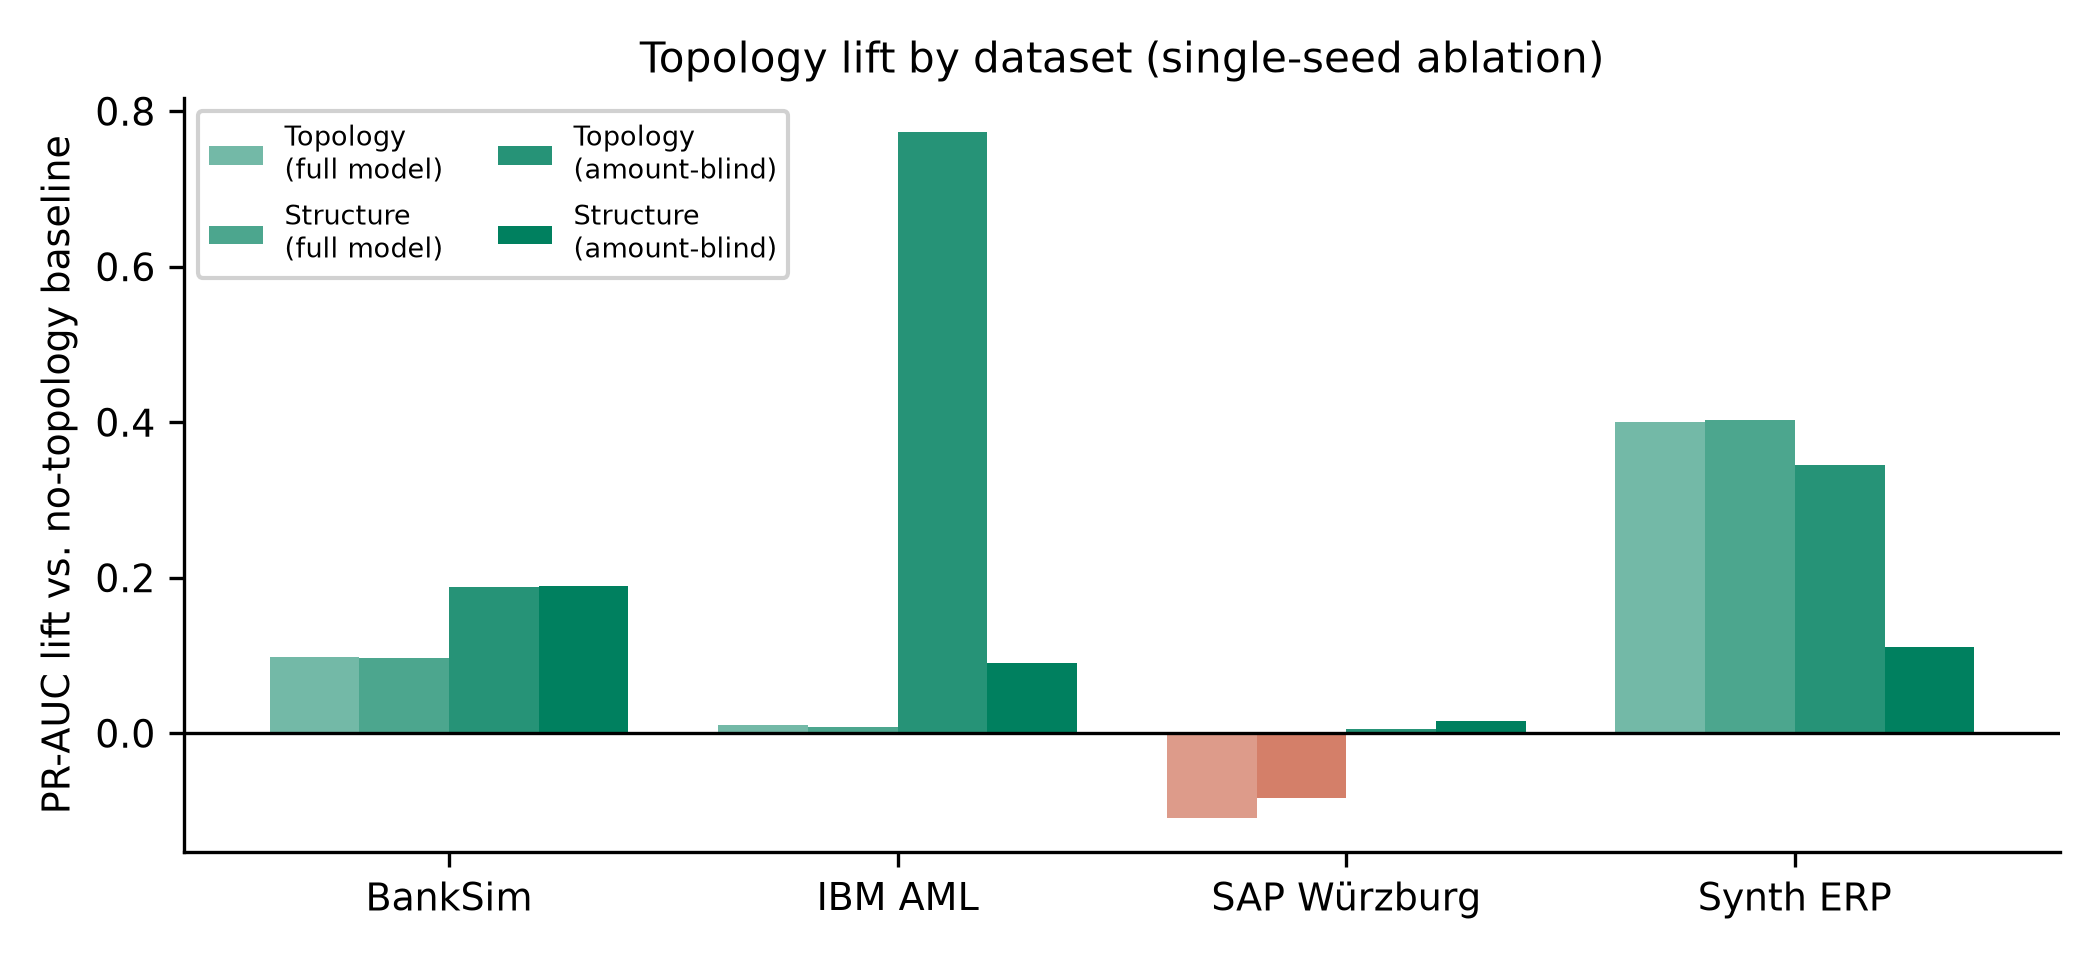
\includegraphics[width=\columnwidth]{figures/ablation_lift_by_dataset.png}
\caption{The four lift statistics of Table~\ref{tab:ablation-lifts} plotted by dataset, making visually explicit that SAP W\"urzburg is the only dataset where both full-model lifts are negative while its two amount-blind lifts remain (barely) positive.}
\label{fig:ablation-lift-by-dataset}
\end{figure}

\subsubsection{Dataset-by-dataset verdict}
\textbf{BankSim: yes.} The full-model structure lift is $+0.0974$ PR-AUC (an $11.7\%$ relative improvement over the $0.833$ baseline, $0.0974/0.833$), and — decisively — the clean amount-blind probe confirms it independently: with every amount feature removed from both sides of the comparison, pure structure still adds $+0.1899$ PR-AUC ($0.634 \to 0.824$). BankSim's topology-importance breakdown (\texttt{ablation.json}) attributes this almost entirely to two density features, \texttt{dest\_in\_degree} (gain importance $0.520$) and \texttt{fan\_in} ($0.091$): BankSim transactions run customer $\to$ merchant, so cycles are structurally impossible, and the signal that remains is exactly the "many senders funnel into one receiver" mule-collection pattern the fan-in features are built to detect. This is the cleanest positive result in the ablation, on a real (simulated-but-not-synthetic-generated) dataset, under both the contaminated and the clean test.

\textbf{IBM~AML: uninformative in the full model; the real signal is elsewhere.} The ordinary baseline alone already reaches PR-AUC $0.990$, leaving essentially no headroom: the full-model structure lift of $+0.0079$ is small in both absolute and relative terms, and — as \S\ref{sec:ablation-stats} makes explicit — falls below this project's own single-seed noise floor, so it cannot be read as evidence of anything. The dirty amount-blind topology probe reaches a striking PR-AUC of $0.867$ ($+0.7735$ lift over the amount-blind baseline's $0.093$), but this number is not evidence for structure: \texttt{topology\_importance} shows \texttt{lap\_out\_recur} ($0.540$) and \texttt{lap\_out\_payees} ($0.420$) together account for $96\%$ of the gain inside that arm, and both are the amount-derived lapping features excluded from the pure-structure set. The clean amount-blind structure probe — the only honest version of this test — reaches PR-AUC $0.184$, a lift of $+0.0905$ over the $0.093$ amount-blind baseline: real, but an order of magnitude smaller than the $0.867$ figure a less careful ablation would have reported as "topology's contribution." In short: IBM~AML's frauds are given away by recurring near-equal amounts (a re-encoded amount signal, not a graph shape), a finding this project's own earlier probing flagged as refuting its initial premise that IBM~AML would be the decisive topology testbed.

\textbf{SAP W\"urzburg: no — topology actively hurts.} Both full-model lifts are negative: $-0.1090$ for all topology, $-0.0829$ for pure structure alone (\texttt{marginal\_structure\_lift = -0.08288}, the number this project's own methodology rules single out as never to be softened or omitted). Adding any topology columns to the ordinary baseline drives test PR-AUC down from $0.155$ to $0.072$ (structure) or $0.046$ (all topology) — a genuinely negative result, not merely a null one. The two amount-blind lifts are small and positive ($+0.0056$, $+0.0153$), but both baselines they are measured against are themselves extremely weak (PR-AUC $0.049$), so this offers no rehabilitation. SAP W\"urzburg is also the one dataset in this study with only $25$ test-split frauds, which we treat as a hard interpretability ceiling rather than a footnote: with that few positive examples, a handful of ranking swaps can move PR-AUC by tens of a point, and \S\ref{sec:ablation-stats} presents an independent, multi-seed confirmation that this dataset's metrics are indeed unstable. We report the negative result plainly rather than either suppressing it or explaining it away, while being explicit that "topology hurts here" and "this measurement is high-variance" are both true simultaneously.

\textbf{Synth-ERP: yes, the largest lift measured — and the one result that cannot be used as thesis evidence.} The full-model structure lift is $+0.4031$ PR-AUC, a $246.8\%$ relative improvement over a weak $0.163$ baseline, with a clean amount-blind confirmation of $+0.1115$. This is real signal by every measure this ablation applies. It is also, definitionally, the least informative result for the paper's actual scientific claim: synth\_erp is this project's own generated dataset, built and calibrated specifically to have rich, ERP-flavored graph structure, and the project's binding policy (adopted precisely to avoid grading its own homework) treats it as a training/stress-testing corpus only, never as evidence that topology helps on real transaction data. We report the number because it is honest and instructive about what topology \emph{can} do when a dataset is constructed to contain strong structural fraud signatures — but it answers a different, narrower question than the one this section opened with.

\subsubsection{Statistical caveats: one seed, no confidence intervals, and a stated noise floor}\label{sec:ablation-stats}
Every number in Tables~\ref{tab:ablation-arms} and \ref{tab:ablation-lifts} comes from a single training run per arm (seed 42), not an average over repeated runs. \texttt{ablation.json} carries no standard deviations, no confidence intervals, and no significance tests, and none should be inferred from it. This project's own training harness documents its rationale for treating small single-seed margins with suspicion: per the comment in \texttt{src/modeling/harness.py}, "single-seed differences of $\sim$0.01 PR-AUC are within XGBoost's subsample noise," and \texttt{experiments/ablation.py}'s own verdict logic uses exactly this $0.01$ figure as the cutoff below which a lift is characterized as "adds $\sim$nothing" rather than a genuine effect. By this project's own stated standard, IBM~AML's full-model structure lift of $+0.00792$ is below the noise floor and is not distinguishable from zero on the evidence of a single seed — a second, independent reason (beyond baseline saturation) that the IBM~AML full-model comparison cannot be read as informative.

A separate, multi-seed experiment offers some corroborating context, though it is not a like-for-like repetition of the arms above: \texttt{final\_champions.json} trains each dataset's final champion configuration — ordinary $+$ topology $+$ TGN embeddings, a superset of the ablation's \emph{+Structure} arm that additionally includes the 65-dimensional temporal-graph-network features discussed elsewhere in this paper — three times, with seeds $\{42,43,44\}$, and reports mean $\pm$ standard deviation. Its per-dataset stability is informative about exactly the concern raised above: BankSim's three-seed test PR-AUC is $0.9364 \pm 0.0015$ (a $0.16\%$ relative standard deviation), consistent with this dataset's ranking being robust to seed choice; SAP W\"urzburg's is $0.1557 \pm 0.0717$ — a $46\%$ relative standard deviation on the mean — which independently corroborates, from a completely different experiment and feature set, the instability that the ablation's own 25-test-fraud caveat already predicts. SAP W\"urzburg's imbalance-mechanism selection for this same champion run is explicitly flagged \texttt{reliable:~false}, and its hyperparameter search was skipped altogether (validation frauds below the guard threshold described in \S\ref{sec:protocol}), so its champion runs on the harness's locked default configuration rather than a tuned one. None of this changes the ablation's central negative finding for SAP W\"urzburg — if anything it strengthens the case for treating that finding as directionally real but numerically imprecise, exactly as reported above — but it is a materially different, TGN-inclusive experiment and its numbers should not be conflated with the seed-42-only ablation arms in Tables~\ref{tab:ablation-arms}--\ref{tab:ablation-lifts}. We also note, to keep every PR-AUC in this paper unambiguous: the champion figures cited in this paragraph describe the offline, research-only model family evaluated for this ablation and are not the model served by the production audit console, which for latency and reproducibility reasons excludes the TGN component; that distinction is maintained precisely wherever this paper reports a PR-AUC for a specific model.

\subsubsection{The cycle-feature paradox}
The project's topology engine was built around five detectors intended to be its signature contribution — \texttt{in\_cycle}, \texttt{cycle\_length}, \texttt{in\_cycle\_ge3}, \texttt{cycle\_amount\_ratio}, and \texttt{cycle\_time\_span} — measuring whether a transaction closes a money loop, how long that loop is, and how tightly it conserves the amount that entered it. The ablation's own gain-importance breakdown does not support these as the load-bearing signal. Table~\ref{tab:cycle-importance} sums the gain importance of all five cycle features, within the full \emph{+Topology} model, against the single highest-importance density feature on the same dataset. On three of the four datasets — BankSim, IBM~AML, and SAP W\"urzburg — every one of the five cycle features scores exactly $0.0$ gain importance; the model finds no split in five hundred boosting rounds for which distinguishing "closes a 3-hop cycle" from "does not" reduces loss more than an already-available split on in-degree, fan-in, or (on IBM~AML) the amount-derived lapping columns. Only on synth\_erp — the one dataset engineered specifically to contain rich cyclic laundering structure — do the cycle features register non-zero importance, and even there their combined mass ($0.0275$) is roughly a third of the single top feature, \texttt{src\_out\_degree} ($0.0786$).

\begin{table}[t]
\centering
\caption{Combined gain importance of the five cycle features vs.\ the single highest-importance density feature, within the baseline+topology model. \texttt{topology\_importance}, \texttt{paper/data/ablation.json}.}
\label{tab:cycle-importance}
\small
\begin{tabular}{lccc}
\toprule
Dataset & $\Sigma$ cycle feats. & Top non-cycle feat. & Importance \\
\midrule
BankSim & 0.0000 & \texttt{dest\_in\_degree} & 0.5199 \\
IBM AML & 0.0018 & \texttt{lap\_out\_recur}$^\dagger$ & 0.5397 \\
SAP W. & 0.0000 & \texttt{fan\_in} & 0.1791 \\
Synth-ERP & 0.0275 & \texttt{src\_out\_degree} & 0.0786 \\
\bottomrule
\end{tabular}
\\[3pt]
\raggedright{\scriptsize $^\dagger$Amount-derived, not pure structure. Among pure-structure features on IBM AML, the top scorer is \texttt{dest\_in\_degree}/\texttt{fan\_in} at $0.0003$.}
\end{table}

%% FIGURE TODO: small-multiples heatmap, one panel per dataset, rows = the 13 topology feature names (grouped visually into the 8 pure-structure and 5 amount-derived features), single column of cell shading by gain importance value from topology_importance in ablation.json, making the "cycle features are a near-empty column on 3 of 4 panels" pattern visible at a glance.
\begin{figure}[t]
\centering
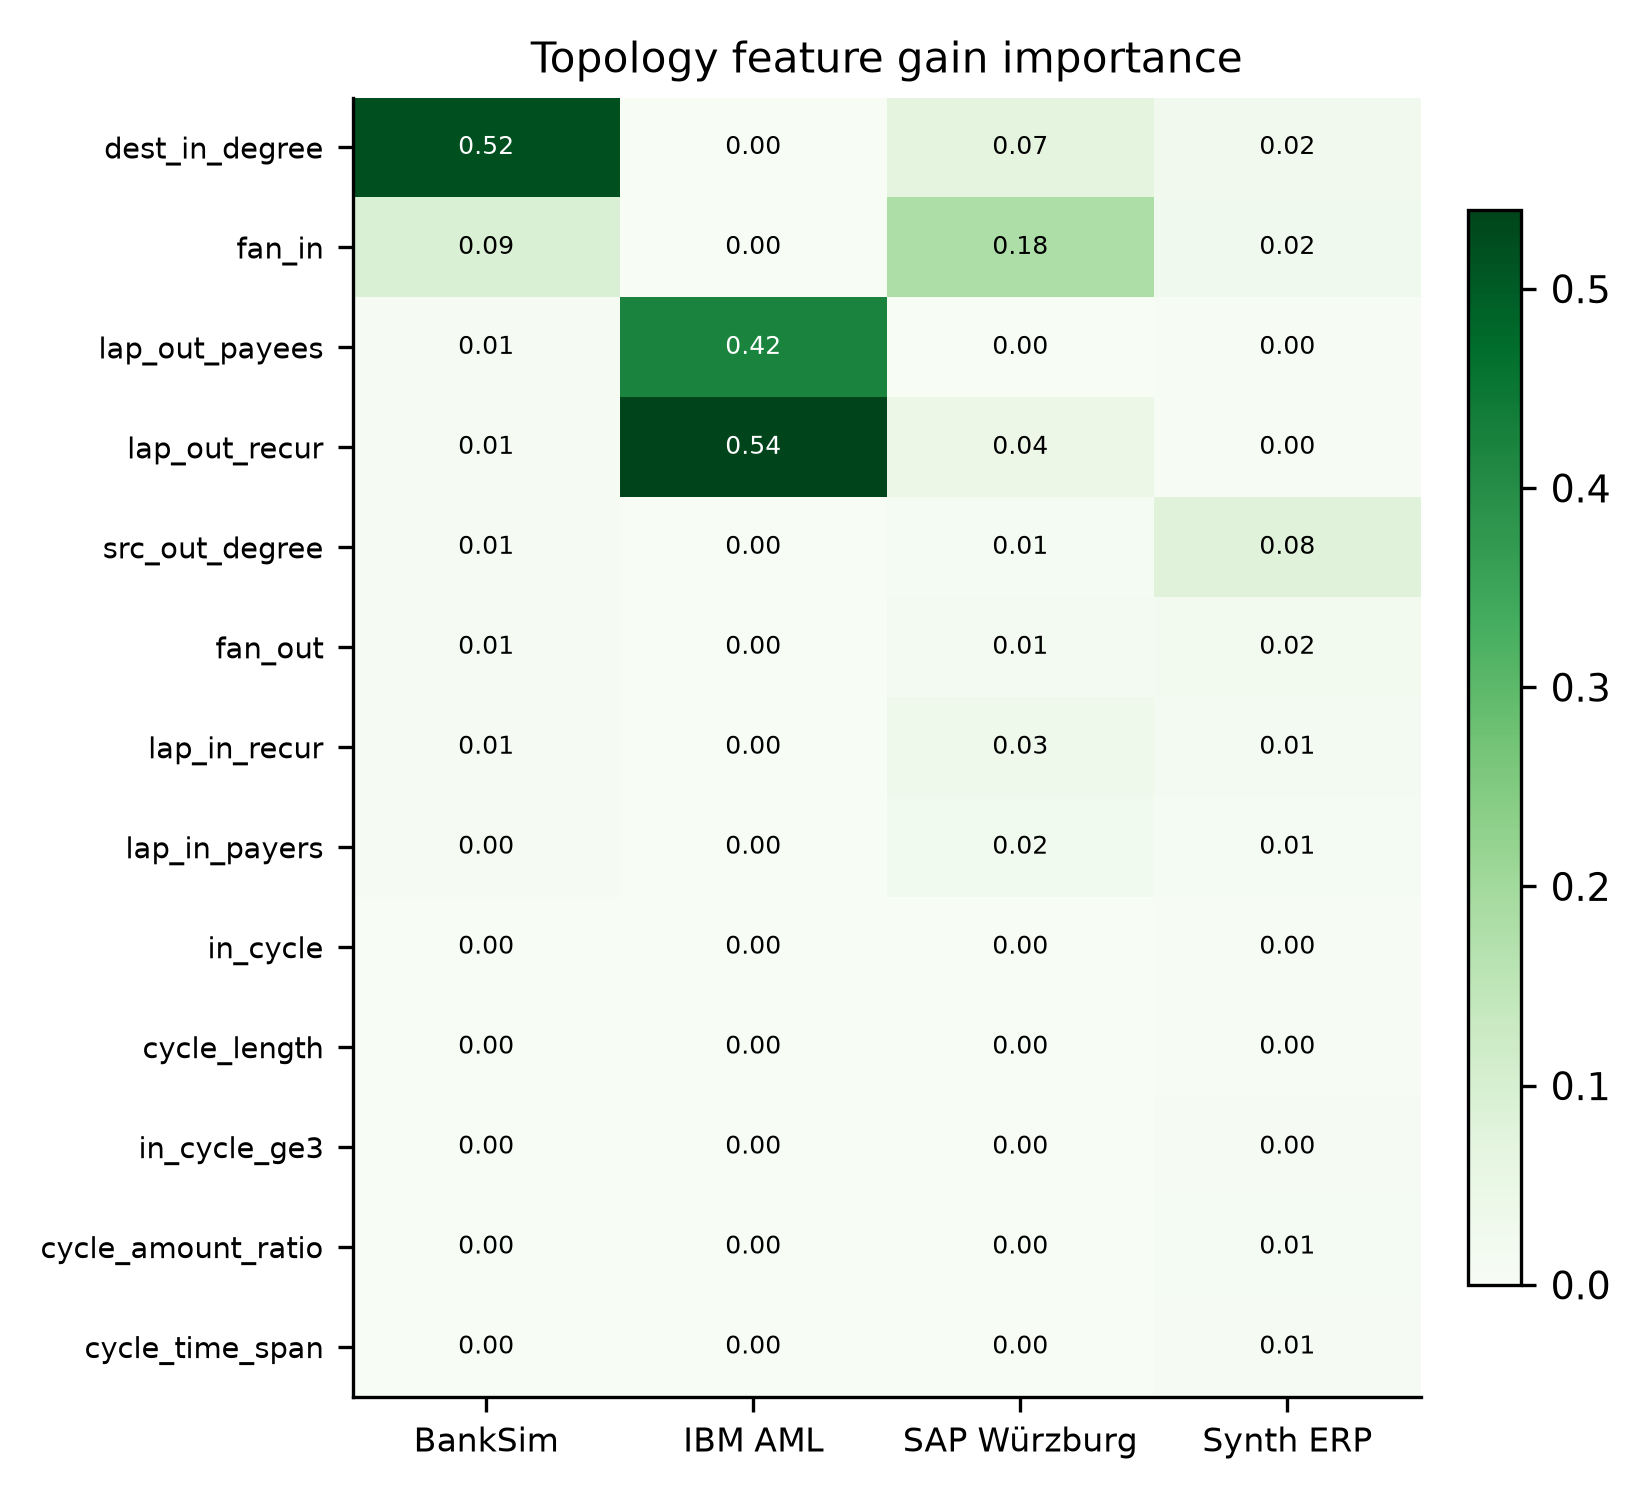
\includegraphics[width=\columnwidth]{figures/topology_importance_heatmap.png}
\caption{Topology feature gain importance by dataset (\texttt{topology\_importance}, Table~\ref{tab:cycle-importance}'s underlying data), grouping pure-structure against amount-derived features and making visible how consistently the five cycle features sit at or near zero while a small number of density features (in-degree, fan-in) or amount-derived lapping features carry essentially all of the mass.}
\label{fig:cycle-heatmap}
\end{figure}


\subsection{Modernization: Focal Loss and Temporal Graph Networks}\label{sec:modern}

The ablation study above establishes, from a single training seed, that hand-crafted topology features carry a leakage-free signal on BankSim and (conditionally) on IBM AML. Two questions remain unanswered by a single seed: whether that signal is robust to run-to-run randomness, and whether a \emph{learned} structural representation --- one that does not depend on the five hand-designed detectors --- can do better. This section reports a second, purpose-built study that answers both. Every arm below is trained with three random seeds (42, 43, 44) and reported as mean $\pm$ standard deviation, the project's own minimum bar for treating a difference as real rather than noise. Two independent upgrades to the locked XGBoost baseline are tested: (1) focal loss~\cite{lin2017focal} as an alternative to class-weighting for handling the $<$1.3\% fraud rate, implemented as a custom, deliberately alpha-free XGBoost~\cite{chen2016xgboost} objective so that it never doubles up with class weights as a second imbalance mechanism; and (2) a Temporal Graph Network (TGN)~\cite{rossi2020temporal}, a self-supervised, label-free encoder that learns a 32-dimensional GRU memory vector per account from the raw transaction stream and emits it, frozen, as 65 additional feature columns (32 source-account dimensions, 32 destination-account dimensions, and one scalar ``edge-expectedness'' score summarizing how surprising the pair is given the account's history). Because it is trained purely as next-link prediction, TGN sees no fraud labels and, following the project's own lapping-detector lesson, is deliberately amount-blind: it observes only who transacted with whom and when.

All results in this section come from \texttt{paper/data/modern.json} (the controlled multi-seed comparison) and \texttt{paper/data/final\_champions.json} (the actual champion-selection pipeline, which additionally runs a light 20-configuration hyperparameter search); numbers drawn from the single-seed ablation study are marked explicitly as such. Four feature-family arms are compared, holding the time-aware splits, XGBoost hyperparameters and (where noted) imbalance mechanism fixed within each comparison: \textbf{A} = ordinary transaction features only (21/8/20/15 features for BankSim/IBM~AML/SAP~Würzburg/synth\_erp); \textbf{B} = A + the 13 hand-crafted topology features; \textbf{C} = A + the 65 TGN columns (no hand-crafted topology); \textbf{D} = A + topology + TGN combined. The 13-feature topology block and 65-feature TGN block are identical in width across all four datasets, which is a useful internal consistency check: $|A|+13+65$ equals the reported full-feature-set size in every case (e.g.\ $21+13+65=99$ for BankSim, $8+13+65=86$ for IBM~AML). The focal-vs-class-weight comparison is run on arms A and B only (both imbalance mechanisms); arms C and D are run with class weights alone, since their purpose is to isolate the marginal value of a learned structural representation, not to re-litigate the imbalance-mechanism question a second time.

One dataset-scope note carries over from the ablation study: SAP Würzburg's splits in this section (120{,}341 / 40{,}114 / 40{,}116 train/val/test, 204/19/25 frauds, taken from \texttt{modern.json} and matching \texttt{final\_champions.json}) are the non-partition-aware split, not the partition-aware split (120{,}411 / 40{,}137 / 40{,}139) used elsewhere in this paper's headline ablation; the two SAP Würzburg number sets should not be pooled.

\subsubsection{Focal loss versus class weights}

Table~\ref{tab:focal-arms} reports the three-seed test PR-AUC for the ordinary-only (A) and ordinary+topology (B) arms under both imbalance mechanisms. Focal loss helps on the ordinary-only baseline in all four datasets, most dramatically on SAP Würzburg (+0.0383) and synth\_erp (+0.1690); once topology is added, its effect is mixed --- a small loss on BankSim ($-0.0060$), a wash on IBM AML (0.0000, both already at the PR-AUC ceiling), a large and volatile gain on SAP Würzburg (+0.2460, on 25 test frauds), and a solid gain on synth\_erp (+0.2014).

\begin{table}[t]
\centering
\caption{Three-seed test PR-AUC, class weights vs.\ focal loss ($\gamma{=}2.0$), ordinary-only (A) and ordinary+topology (B) arms. $\Delta$ = focal $-$ class-weight. $^\dagger$synth\_erp is synthetic and never used as thesis evidence.}
\label{tab:focal-arms}
\resizebox{\columnwidth}{!}{%
\scriptsize
\begin{tabular}{lrrrrrr}
\toprule
Dataset & A$_{cw}$ & A$_{focal}$ & $\Delta_A$ & B$_{cw}$ & B$_{focal}$ & $\Delta_B$ \\
\midrule
BankSim & 0.7870{\tiny$\pm$0.0700} & 0.8616{\tiny$\pm$0.0001} & +0.0746 & 0.9319{\tiny$\pm$0.0017} & 0.9259{\tiny$\pm$0.0008} & $-$0.0060 \\
IBM AML & 0.9920{\tiny$\pm$0.0026} & 0.9968{\tiny$\pm$0.0001} & +0.0048 & 1.0000{\tiny$\pm$0.0000} & 1.0000{\tiny$\pm$0.0000} & 0.0000 \\
SAP Würzburg & 0.1581{\tiny$\pm$0.0129} & 0.1963{\tiny$\pm$0.0252} & +0.0383 & 0.0717{\tiny$\pm$0.0095} & 0.3177{\tiny$\pm$0.1470} & +0.2460 \\
synth\_erp$^\dagger$ & 0.2483{\tiny$\pm$0.0602} & 0.4173{\tiny$\pm$0.0120} & +0.1690 & 0.4569{\tiny$\pm$0.1547} & 0.6583{\tiny$\pm$0.0031} & +0.2014 \\
\bottomrule
\end{tabular}}
\end{table}

The most consequential effect of focal loss, however, is not its mean shift but its effect on \emph{variance}. On BankSim's ordinary-only arm, moving from class weights to focal loss collapses the three-seed standard deviation from 0.0700 to 0.00007 --- roughly three orders of magnitude, from ``a coin-flip's width of uncertainty'' to ``machine-precision-adjacent.'' This is sharpened by comparing against the single-seed ablation study, which reported a BankSim baseline PR-AUC of 0.8330 (\texttt{ablation.json}, seed 42 only, class weights). That single number sits roughly two-thirds of one standard deviation above the three-seed class-weight mean of 0.7870 reported here --- a concrete illustration of why the project's own methodology treats single-seed differences smaller than $\sim$0.01 PR-AUC as noise: an unlucky or lucky seed choice alone can move the class-weighted BankSim baseline by several hundredths. Under focal loss the same arm's three-seed spread (0.8616 $\pm$ 0.00007) makes this kind of seed sensitivity essentially disappear.

This variance-collapsing property is also what wins focal loss its place in the champion pipeline. Table~\ref{tab:champion-selection} reports \texttt{final\_champions.json}'s validation-selection step, which compares the full feature set (A+B+C combined, i.e.\ arm D) under class weights against the same feature set under focal loss and selects whichever wins on validation PR-AUC --- never on test. Focal loss wins the selection on three of the four datasets: BankSim, SAP Würzburg, and synth\_erp; on IBM AML the two mechanisms tie exactly at the saturated ceiling (1.0000 vs.\ 1.0000) and the pipeline's tie-break falls to class weights. Note that this selection step differs from the controlled arm-D comparison in that it also runs a 20-configuration hyperparameter search per candidate (skipped only for SAP Würzburg, whose validation fraud count trips the pipeline's own small-sample guard), so its validation numbers are close to, but not identical with, the fixed-hyperparameter arm-D numbers reported elsewhere in this section --- for example BankSim's tuned class-weight validation PR-AUC is 0.9489 versus the fixed-hyperparameter arm D's 0.9426.

\begin{table}[t]
\centering
\caption{Champion validation selection (\texttt{final\_champions.json}), full feature set (topology+TGN+ordinary). Margin = focal $-$ class-weight on validation. $^\ddagger$selection flagged \texttt{reliable=false} (SAP Würzburg's HPO was skipped by the small-sample guard). $^\dagger$synth\_erp is non-evidentiary.}
\label{tab:champion-selection}
\resizebox{\columnwidth}{!}{%
\scriptsize
\begin{tabular}{lrrlrr}
\toprule
Dataset & Val (cw) & Val (focal) & Winner (margin) & Test (cw) & Test (focal) \\
\midrule
BankSim & 0.9489{\tiny$\pm$0.0009} & 0.9515{\tiny$\pm$0.0007} & focal (+0.0026) & 0.9395{\tiny$\pm$0.0006} & 0.9364{\tiny$\pm$0.0015} \\
IBM AML & 1.0000{\tiny$\pm$0.0000} & 1.0000{\tiny$\pm$0.0000} & cw (tie, 0.0000) & 1.0000{\tiny$\pm$0.0000} & 1.0000{\tiny$\pm$0.0000} \\
SAP Würzburg & 0.2888{\tiny$\pm$0.0436} & 0.3562{\tiny$\pm$0.0195} & focal$^\ddagger$ (+0.0674) & 0.1401{\tiny$\pm$0.0076} & 0.1557{\tiny$\pm$0.0717} \\
synth\_erp$^\dagger$ & 0.8487{\tiny$\pm$0.0017} & 0.8507{\tiny$\pm$0.0025} & focal (+0.0020) & 0.7722{\tiny$\pm$0.0014} & 0.7785{\tiny$\pm$0.0053} \\
\bottomrule
\end{tabular}}
\end{table}

BankSim deserves a specific flag: its validation margin, +0.0026 PR-AUC, is the thinnest \emph{reliable, non-saturated, real-data} margin in the entire selection table --- synth\_erp's nominal margin (+0.0020) is numerically smaller but is excluded from thesis claims as synthetic data, and IBM AML's margin is a literal zero-width tie on an already-saturated metric, not a genuine comparison. A margin this thin, on the dataset the project treats as its cleanest structural-signal testbed, does not survive contact with the test set: the class-weight arm actually scores higher on BankSim's held-out test period (0.9395 $\pm$ 0.0006) than the focal arm that was selected on validation (0.9364 $\pm$ 0.0015), a reversal of 0.0032 PR-AUC. We report this plainly as a caution against over-reading small validation margins, per the project's own threshold-freezing discipline; it does not overturn the selection (validation-only selection is the whole point of never touching test until after the choice is frozen), and it is operationally invisible at the metric an auditor actually cares about --- precision@100 is 1.00 for both arms.

\subsubsection{Temporal graph network embeddings}

Table~\ref{tab:tgn-lift} isolates the value of the learned TGN representation against two references: the ordinary-only baseline (arm C $-$ arm A, both class-weighted) and the hand-crafted topology block (arm C $-$ arm B), plus the incremental value of combining both representations (arm D $-$ arm B) and TGN's share of total SHAP feature importance in the champion model (from \texttt{final\_champions.json}'s per-dataset SHAP summary).

\begin{table}[t]
\centering
\caption{TGN embeddings vs.\ hand-crafted topology, 3-seed test PR-AUC deltas (class-weighted arms only) and TGN's share of total SHAP importance in the champion model. $^\dagger$synth\_erp is non-evidentiary.}
\label{tab:tgn-lift}
\resizebox{\columnwidth}{!}{%
\scriptsize
\begin{tabular}{lrrrr}
\toprule
Dataset & TGN$-$base. & TGN$-$topo. & Comb.$-$topo. & TGN SHAP share \\
\midrule
BankSim & +0.1326 & $-$0.0123 & +0.0004 & 17.5\% \\
IBM AML & $-$0.0048 & $-$0.0128 & 0.0000 & 1.9\% \\
SAP Würzburg & $-$0.0987 & $-$0.0124 & +0.0684 & 42.0\% \\
synth\_erp$^\dagger$ & +0.4489 & +0.2404 & +0.2850 & 37.3\% \\
\bottomrule
\end{tabular}}
\end{table}

The central, load-bearing finding of this table is the middle column. On every real dataset, TGN alone (arm C) scores \emph{below} hand-crafted topology alone (arm B): $-$0.0123 on BankSim, $-$0.0128 on IBM AML, $-$0.0124 on SAP Würzburg. These three deltas are remarkably tight given how different the three datasets are in scale, fraud rate, and graph density --- all three cluster within 0.0005 of $-$0.0125. Learned, self-supervised structural embeddings simply do not beat five purpose-built, domain-informed detectors on real transaction graphs in this study; the only dataset where TGN outperforms hand-crafted topology is synth\_erp (+0.2404), the project's own synthetic environment, which is explicitly excluded from evidentiary claims (Section~\ref{sec:threats}). The first column tells a related but distinct story: TGN's lift over the plain ordinary-feature baseline is positive on BankSim (+0.1326, nearly matching topology's own +0.1449 lift there) but slightly \emph{negative} on both IBM AML ($-$0.0048) and SAP Würzburg ($-$0.0987). On IBM AML this is a small movement within noise (both arms sit near the saturated ceiling, std $\approx$0.01); on SAP Würzburg it is a large, consistent penalty, echoing the same dataset's negative topology lift reported in the ablation study --- on this small, thin ERP ledger, adding structural feature complexity of either kind tends to hurt rather than help, plausibly because 25 test frauds cannot support the additional degrees of freedom either representation introduces.

Combining topology and TGN (arm D vs.\ arm B) adds negligible value beyond topology alone on the two datasets with the cleanest signal: +0.0004 on BankSim, 0.0000 on IBM AML (already saturated). SAP Würzburg's combined arm does show a nominal +0.0684 recovery over its topology-only arm, but this sits inside the same small-sample volatility that produced SAP's other large, sign-flipping deltas in this section and should not be read as evidence that TGN rescues topology's failure there. synth\_erp's large combined gain (+0.2850) is, again, a synthetic-data result only.

This pattern is consistent with, not contradicted by, the 2026 literature on graph-native alternatives: Lei et al.'s STC-MixHop~\cite{lei2026stcmixhop} reports the same qualitative result on a different transaction-fraud benchmark, that a graph-learning architecture struggles to outperform a tabular baseline once node attributes already carry strong signal, and attributes graph structure's value specifically to settings where relational patterns are operationally significant rather than universal. This paper's own dataset-by-dataset TGN comparison is, in effect, an independent empirical instance of exactly that claim: TGN loses to hand-crafted topology on every real dataset in this study, each of which differs in scale, fraud rate, and graph density, and wins only on the one dataset (\texttt{synth\_erp}) explicitly engineered to have rich, easily learnable structure.

A last observation cautions against reading SHAP importance share as a proxy for ablation-validated value. SAP Würzburg's TGN block claims the \emph{largest} share of total SHAP importance of any dataset in this study (42.0\%) despite producing the study's most negative TGN lift ($-$0.0987 over baseline, $-$0.0124 over topology); IBM AML shows the opposite pattern, with TGN carrying almost no importance (1.9\%) on a baseline it also fails to improve. A feature family can dominate a model's internal attribution and still not earn its place in a leakage-free ablation --- the same lesson the ablation study draws for hand-crafted cycle features applies here to a learned representation as well, via TreeSHAP's exact per-feature attribution~\cite{lundberg2017unified,lundberg2020local}.

%% FIGURE TODO: grouped bar chart, one group per dataset (BankSim, IBM AML, SAP Würzburg, synth_erp), two bars per group showing tgn_vs_handcrafted_topology and combined_vs_topology (PR-AUC delta, signed, with a zero reference line), to make visually obvious that the "TGN vs topology" bar is negative on all three real datasets and positive only on synth_erp.
\begin{figure}[t]
\centering
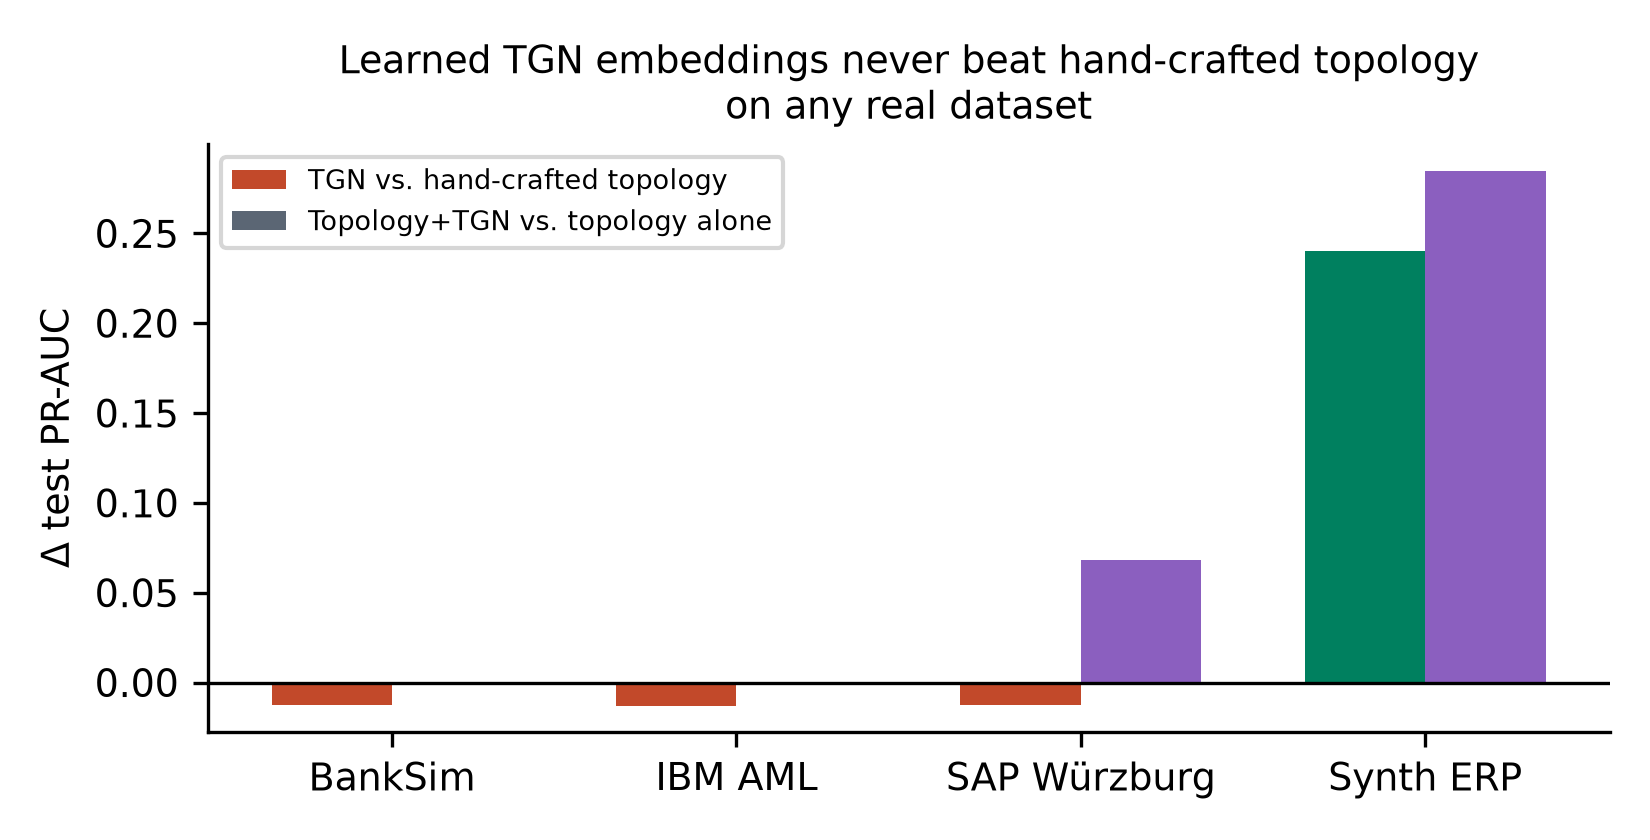
\includegraphics[width=\columnwidth]{figures/modern_tgn_lift_by_dataset.png}
\caption{TGN-vs-topology and combined-vs-topology PR-AUC deltas by dataset (\texttt{modern.json}). The TGN-vs-topology bar is negative on all three real datasets and positive only on the non-evidentiary synth\_erp dataset.}
\label{fig:tgn-lift}
\end{figure}

\subsubsection{Implication for the production system}

Two independent findings close off TGN as a candidate for the served model, both already on the record from this build. First, TGN training is not bit-reproducible across machines even with a fixed seed: re-running the TGN trainer on freshly downloaded copies of the same source data and re-scoring against the committed champion bundle does not reproduce the committed test PR-AUC --- BankSim recomputes to 0.845 against the bundle's recorded 0.938, and SAP Würzburg to 0.098 against the bundle's 0.140 (Section~\ref{sec:threats}, Threats to Validity). Small floating-point differences in CPU-side PyTorch training compound across epochs and propagate through a feature block that carries 17--42\% of the champion model's total SHAP importance (Table~\ref{tab:tgn-lift}), so an offline champion bundle trained on one machine cannot be assumed to reproduce its recorded score on another. Second, and independently disqualifying, the TGN's per-account GRU memory tensor --- the running state that makes its embeddings meaningful at any given point in time --- is never persisted by the training code; it exists only inside the training process and is discarded on exit, so there is no artifact from which a live scoring service could resume the memory a freshly arriving transaction would need.

For these reasons, the production system described in Section~\ref{sec:production} does not serve the TGN-augmented champion at all. It serves a separate, explicitly named \emph{online} bundle --- ordinary features plus hand-crafted topology only, arm B's feature set --- built and reported independently in \texttt{paper/data/online\_bundles.json}: 34 features and test PR-AUC 0.9311 $\pm$ 0.0005 on BankSim, 33 features and 0.1094 $\pm$ 0.0198 on SAP Würzburg, and 28 features and 0.5702 $\pm$ 0.0174 on synth\_erp. IBM AML's online-bundle entry, labeled \texttt{ibm\_aml\_kaggle} (26 features, test PR-AUC 0.5120 $\pm$ 0.0674), is a fresh Kaggle re-download reproduction check, not the same simulator instance behind this section's headline IBM AML numbers, and its PR-AUC is correspondingly far below this section's saturated 1.0000 --- a difference of instance, not of method, and one more reason the two IBM AML number sets in this paper must never be merged. In short: every PR-AUC reported in this section for the ``champion'' or ``combined'' arm describes an offline, research-only model; the number that describes what a live transaction would actually be scored against is the online-bundle figure above, and it excludes TGN entirely.

\subsection{Synthetic Economy: Realism and Augmentation Results}
\label{sec:synthetic-realism}

For every statistic we report on \texttt{synth\_erp}, we ask one question:
does it fall inside the range spanned by the four real datasets
(\texttt{ibm\_aml}, \texttt{banksim}, \texttt{sap\_wurzburg}, \texttt{paysim}),
measured with identical methodology, or outside it? Table~\ref{tab:synth-realism}
answers this for six statistics drawn from \texttt{calibration\_reference.json}
and \texttt{synth\_erp\_realism.json}. The fraud rate, the repeat-pair share
of transactions, and the sender/receiver namespace overlap all land inside
the real span. Three do not, and we report them plainly rather than tuning
them away. Log-amount dispersion (\texttt{log1p\_std} = 2.3256) sits above
every real dataset (span 0.9551--2.0193): the simulated economy mixes
cents-scale retail tickets with treasury sweeps of hundreds of thousands of
dollars in one distribution, a wider mixture than any single-domain real
dataset exhibits — genuine \emph{over}-dispersion, not a defensible match.
Benford mean-absolute-deviation (\texttt{benford\_mad} = 0.0047) is
\emph{lower} than every real dataset (span 0.0142--0.0758): \texttt{synth\_erp}'s
amounts obey Benford's law more cleanly than any real ledger we measured,
itself a realism failure in the opposite direction — real accounting data
carries idiosyncratic roundness and human-entered biases that a mixture of
lognormal generators does not reproduce. Pair reciprocity
(\texttt{pair\_reciprocity} = 0.1356) is roughly $3.0\times$ the real maximum
(0.0446, \texttt{ibm\_aml}): salary-to-purchase circulation and refund/cover
behavior generate more back-and-forth pairs than any of the four real
economies structurally permit. None of these three deviations is hidden in
downstream use: they are why \texttt{synth\_erp} is never treated as evidence
for this paper's central topology claim, only as training material and a
stress test, per the usage policy at the top of this section.

%% FIGURE TODO: grouped bar chart with one bar-triplet per calibration metric
%% (fraud rate, log1p_std, benford_mad, pair_reciprocity, repeat_pair_frac,
%% namespace_overlap): synth_erp value vs. the real-dataset min-max band
%% (shown as a shaded range or error bar), so in-range vs. out-of-range
%% metrics are visually obvious at a glance. Omitted from the body to save
%% space given Table~\ref{tab:synth-realism} already reports the same numbers.

\begin{table}[t]
\centering
\small
\caption{Realism audit: \texttt{synth\_erp} vs.\ the real-dataset reference band (min--max across \texttt{ibm\_aml}, \texttt{banksim}, \texttt{sap\_wurzburg}, \texttt{paysim}). Source: \texttt{calibration\_reference.json}, \texttt{synth\_erp\_realism.json}.}
\label{tab:synth-realism}
\resizebox{\columnwidth}{!}{%
\begin{tabular}{@{}lrrrl@{}}
\toprule
Metric & \texttt{synth\_erp} & Real min & Real max & In band? \\
\midrule
Fraud rate               & 0.4884\% & 0.1236\% & 1.2108\% & Yes \\
Repeat-pair txn.\ share  & 0.8586   & 0.0      & 0.9936   & Yes \\
Namespace overlap        & 0.9410   & 0.0      & 0.9927   & Yes \\
log1p(amount) std.\      & 2.3256   & 0.9551   & 2.0193   & \textbf{No (above)} \\
Benford MAD              & 0.0047   & 0.0142   & 0.0758   & \textbf{No (below)} \\
Pair reciprocity         & 0.1356   & 0.0      & 0.0446   & \textbf{No (3.0$\times$ above)} \\
\bottomrule
\end{tabular}%
}
\end{table}

A more direct realism concern is whether fraud amounts alone give fraud away —
the specific artifact this project identified in \texttt{ibm\_aml} elsewhere in
this paper (fraud amounts distinctively \emph{small}, amount-ratio 0.068,
globally separable at ROC-AUC $\approx 0.91$). On \texttt{synth\_erp}, the
median fraud amount (\$1{,}692.59) is 23.79$\times$ the median benign amount
(\$71.14; the equivalent ratio in \texttt{banksim}, from
\texttt{calibration\_reference.json}, is 11.9$\times$), and a univariate
log-amount classifier reaches ROC-AUC 0.8078 overall (KS statistic 0.604
between the fraud and benign log-amount distributions) — at first glance a
fraud population skewed to B2B-sized amounts in a retail-heavy economy.
Restricted to the amount band where 93\% of fraud actually lives
(\$300--\$20{,}000, $n=5{,}228$ fraud rows in band), that same classifier
collapses to ROC-AUC 0.4911 — indistinguishable from chance. Fraud amounts
are globally distinguishable only because fraud skews toward a coarser amount
regime than the bulk of retail traffic; \emph{within} its own regime, amount
carries essentially no signal, forcing any detector toward behavioral or
structural evidence rather than a one-column amount rule — the opposite of
the \texttt{ibm\_aml} artifact, and a deliberate design target corroborated
here after the fact rather than asserted in advance.

\subsubsection{Adversarial Tabular-Leak Probe}
\label{sec:synthetic-leakprobe}

A realistic amount distribution does not rule out a cheap categorical
shortcut elsewhere in the table — the same class of hidden bias that motivates
auditing tabular fraud-evaluation datasets for shortcut features before
trusting them~\cite{jesus2022turning}. We therefore ran an automated probe over 16
candidate rules — every \texttt{tx\_type} indicator, an account-creation-date
indicator on each side of the transaction, and pairwise conjunctions of the
two — scoring each rule's support, precision, recall of fraud, and lift over
the 0.4884\% base rate. Table~\ref{tab:synth-leakprobe} reports the eight
highest-lift rules out of the 16 tested. Three flow types
(\texttt{tx\_type=payroll}, \texttt{tx\_type=recurring\_bill},
\texttt{tx\_type=refund}) and their conjunctions with a mid-year account
carry \emph{zero} fraud whatsoever (lift 0.0) — no scenario in the generator
routes any of the five typologies onto these three rails at all, which is a
genuine (if narrow) gap in coverage rather than a realism strength.

The rule the probe itself records as worst,
\texttt{tx\_type=transfer \& dest\_created\_midyear}, reaches a lift of
$19.0\times$ the base rate, support of 26{,}420 transactions, precision of
9.29\%, and recovers 43.75\% of all fraud in a single two-clause rule. The
dataset's own automated gate does not classify this as a leak
(\texttt{leak\_flag} = \texttt{false}, its precision bar sitting well above
what this rule reaches), and a rule flagging under 10\% of the transactions it
fires on as fraud is far from the near-deterministic, one-line shortcuts the
generator's earlier drafts contained before an adversarial review removed
them. Still, a rule with 19$\times$ lift and 44\% recall is a real,
exploitable regularity, not a non-finding, and we report it rather than let a
binary pass/fail flag stand in for a reader's own judgment of where
``legitimate risk factor'' ends and ``tabular leak'' begins. A transaction
moving through the \texttt{transfer} rail toward an account opened within the
same year is a defensible real-world risk heuristic — mid-year account
creation correlates with fraud in practice, not only in this simulation — but
we flag it here precisely so that any model trained on \texttt{synth\_erp}
can be checked for whether it quietly learned this shortcut instead of the
intended structural and behavioral signal.

\begin{table}[t]
\centering
\scriptsize
\caption{Adversarial tabular-leak probe, top 8 of 16 rules by lift. Base fraud rate 0.4884\%. Source: \texttt{synth\_erp\_realism.json}, \texttt{tabular\_leak\_probe}.}
\label{tab:synth-leakprobe}
\resizebox{\columnwidth}{!}{%
\begin{tabular}{@{}lrrrr@{}}
\toprule
Rule & Support & Precision & Recall & Lift \\
\midrule
\texttt{transfer \& dest\_midyear}$^\dagger$ & 26{,}420 & 0.0929 & 0.4375 & \textbf{19.0} \\
\texttt{dest\_created\_midyear}         & 67{,}621  & 0.0502 & 0.6049 & 10.3 \\
\texttt{tx\_type=transfer}              & 94{,}781  & 0.0385 & 0.6500 & 7.9 \\
\texttt{vendor\_payment \& dest\_midyear}$^\dagger$ & 25{,}781 & 0.0316 & 0.1451 & 6.5 \\
\texttt{sale \& dest\_midyear}$^\dagger$          & 8{,}131   & 0.0146 & 0.0212 & 3.0 \\
\texttt{src\_created\_midyear}          & 156{,}550 & 0.0113 & 0.3147 & 2.3 \\
\texttt{reimbursement \& dest\_midyear}$^\dagger$ & 741       & 0.0081 & 0.0011 & 1.7 \\
\texttt{tx\_type=reimbursement}         & 12{,}236  & 0.0079 & 0.0173 & 1.6 \\
\bottomrule
\end{tabular}%
}
\vspace{2pt}
\raggedright\scriptsize $^\dagger$\texttt{dest\_midyear} abbreviates \texttt{dest\_created\_midyear}.
\end{table}

\subsubsection{The Augmentation Transfer Probe}
\label{sec:synthetic-augmentation}

The realism and leak audits above establish what \texttt{synth\_erp} is
calibrated well enough to be used \emph{for}. The most direct test of the
narrower, practical question — does adding \texttt{synth\_erp} rows to a real
dataset's training split make its fraud model better? — is a paired
augmentation experiment: for each of three real datasets, train an XGBoost
model~\cite{chen2016xgboost} three ways (real data only; real data with all
1{,}148{,}503 \texttt{synth\_erp} rows pooled into the training split; and
\texttt{synth\_erp} data only, evaluated zero-shot on the real test split),
each averaged over three seeds, under the same time-aware split, class-weight
imbalance handling, and validation-tuned threshold used throughout this paper.
Table~\ref{tab:synth-augmentation} reports the result, and it is unambiguous:
pooling synthetic rows into training \emph{hurts} test PR-AUC on every one of
the three real datasets tested. \texttt{banksim} falls from
$0.8669\pm0.0031$ (real-only) to $0.7610\pm0.0022$ (real+synth), a paired
per-seed delta of $-0.1059\pm0.0011$; \texttt{ibm\_aml} falls from an
already-saturated $0.99999\pm0.00001$ to $0.9954\pm0.0013$,
$\Delta=-0.0046\pm0.0013$ — small in absolute terms, but the baseline leaves
almost no headroom to fall into, so even this small drop is a consistent,
same-direction result; and \texttt{sap\_wurzburg} — on only 25 test-set
frauds, the same small-sample caveat that applies to every
\texttt{sap\_wurzburg} result in this paper — falls from $0.1366\pm0.0446$ to
$0.0293\pm0.0033$, $\Delta=-0.1073\pm0.0417$.
The mechanism is unsurprising in hindsight given Sec.~\ref{sec:synthetic-realism}:
a single tree ensemble fit jointly over two economies with measurably
different amount dispersion and reciprocity structure pulls its splits toward
the pooled distribution, at the real dataset's expense. We report this as a
clean negative result rather than qualify it away: \emph{naive} pooled
augmentation with this dataset, under this protocol, does not help, on any
real dataset we tested it against.

\begin{table}[t]
\centering
\small
\caption{Augmentation transfer probe: XGBoost PR-AUC, 3-seed mean $\pm$ std. \texttt{synth\_only} is zero-shot (trained solely on \texttt{synth\_erp}, evaluated on the real test split). Source: \texttt{augmentation.json}.}
\label{tab:synth-augmentation}
\resizebox{\columnwidth}{!}{%
\begin{tabular}{@{}lrrrr@{}}
\toprule
Dataset & Real-only & Real+synth & $\Delta$ & Synth-only \\
\midrule
\texttt{banksim} ($n{=}1320$)      & 0.8669$\pm$0.0031 & 0.7610$\pm$0.0022 & $-$0.1059$\pm$0.0011 & \textbf{0.7243$\pm$0.0079} \\
\texttt{ibm\_aml} ($n{=}377$)      & 0.99999$\pm$0.00001 & 0.9954$\pm$0.0013 & $-$0.0046$\pm$0.0013 & 0.0017$\pm$0.0006 \\
\texttt{sap\_wurzburg} ($n{=}25$)  & 0.1366$\pm$0.0446 & 0.0293$\pm$0.0033 & $-$0.1073$\pm$0.0417 & 0.0008$\pm$0.0001 \\
\bottomrule
\end{tabular}%
}
\end{table}

There is exactly one genuinely positive number in this experiment, and it is
a narrower, different claim than ``synthetic data helps supervised
training'': the \texttt{synth\_only} zero-shot column for \texttt{banksim}.
A model that has \emph{never seen a single real BankSim row} — trained
entirely on \texttt{synth\_erp}, evaluated as-is on real, held-out
\texttt{banksim} test data — scores $0.7243\pm0.0079$ PR-AUC, recovering
83.6\% of the $0.8669$ real-trained baseline, at precision@100 of
$0.99\pm0.0082$ against the real-trained baseline's perfect $1.00$; chance at
this split's 1.21\% fraud rate is on the order of $0.01$--$0.02$ PR-AUC, so
this is far from a vacuous transfer. The same zero-shot comparison fails on
\texttt{ibm\_aml} ($0.0017$ PR-AUC against a $0.99999$ real-trained ceiling —
unsurprising, since \texttt{ibm\_aml}'s giveaway-small fraud amounts are
inverted relative to \texttt{synth\_erp}'s B2B-skewed fraud) and on
\texttt{sap\_wurzburg} ($0.0008$ PR-AUC, 25 test frauds, too small to support
any transfer claim). We read the \texttt{banksim} result as evidence that the
synthetic economy teaches \emph{transferable structural and behavioral
discrimination} that generalizes to a real domain it structurally resembles —
not as evidence that pooling synthetic rows into a real training set is a
useful augmentation recipe. These are two different claims, only one of which
this experiment supports; we are careful not to let the positive framing of
the zero-shot result launder the negative framing of the pooled-augmentation
result three rows above it.

\subsubsection{Summary and Scope}

\texttt{synth\_erp} is a large, ERP-flavored, multi-typology synthetic ledger
built under a binding non-circularity constraint and audited, after the fact,
against four real datasets on realism, tabular leakage, and downstream
transfer. It matches the real fraud-rate, repeat-pair, and namespace-overlap
bands; it is measurably over-dispersed in amount and reciprocity and
unrealistically Benford-clean relative to every real dataset compared against
it; its cheapest categorical shortcut reaches 19$\times$ lift and 44\% recall
without being flagged as a formal leak, a judgment call we surface rather
than hide; and pooling it into real training data hurts every real dataset's
PR-AUC we tested, its one positive contribution being a narrower zero-shot
transfer result on the one real dataset it structurally resembles.
Consistent with the usage policy stated at the outset, none of this
section's numbers are used anywhere in this paper as evidence for the
central topology claim (Sec.~\ref{sec:ablation}); \texttt{synth\_erp}'s role
is training material, a per-typology stress test, and demo content for the
audit console (Sec.~\ref{sec:system}), never proof.

\subsection{Explainable Audit Alerts: Results}\label{sec:explain-results}
Three of the four datasets reach perfect precision at their operating $k$
(Table~\ref{tab:alert_precision}): every one of BankSim's top 15, IBM AML's
top 20, and synth\_erp's top 20 test-period alerts is a labelled fraud. IBM
AML's 1.00 should not be over-read, however: its baseline model is already
saturated at $\mathrm{PR\text{-}AUC}\approx0.99$ (the ablation study reported earlier in this paper),
so a perfect top-$k$ here is consistent with the amount signal alone doing
the work and does not, on its own, demonstrate that topology mattered for
these particular alerts -- three of the twenty carry no reconstructable
fan-in or cycle evidence at all (\texttt{evidence\_type\_counts.none}=3),
meaning their risk drivers were purely \texttt{ordinary}/\texttt{tgn}.

SAP Würzburg is the outlier the ablation predicts: precision@10 is 0.20 (2 of
10), the weakest by a wide margin, the direct operational consequence of the
dataset's negative marginal structural lift reported elsewhere in this
paper, compounded by only 25 labelled test frauds. Every one of its ten
alerts is nonetheless a syntactically well-formed, replay-verified fan-in --
destinations collecting from 166 to 271 distinct senders in-window --
because those accounts are simply high-traffic general-ledger hubs
(\texttt{GL:895000}, \texttt{GL:300000}), not because fraud is present. This
is the clearest illustration in the paper of what Layer 2 actually
guarantees: the evidence is provably consistent with what the model saw,
never a guarantee that what the model saw was fraud. (Its test-partition
size also differs by source file: \texttt{final\_champions.json}, which
produced this bundle, reports 40{,}116 test rows / 25 frauds, while
\texttt{ablation.json}'s separately-run partition-aware split reports
40{,}139 -- the two pipeline runs are not the same split and should not be
merged.)

\subsubsection{Global Attribution Is Dataset-Specific, Not Universal}
Averaging $|\text{SHAP}|$ over a sample of each dataset's test rows
(\texttt{final\_champions.json}: \texttt{shap\_global\_top20}, 50{,}000
sampled rows for BankSim/IBM~AML/synth\_erp and the full 40{,}114-row test
partition for SAP Würzburg, since \texttt{bundle\_metadata.json} does not
itself carry per-feature magnitudes) shows that no single family dominates
across datasets (Table~\ref{tab:global_shap}).

\begin{table}[t]
\centering
\caption{Top-3 globally attributed features per dataset by mean $|$SHAP$|$ (margin space), with family tag (\texttt{paper/data/final\_champions.json}).}
\label{tab:global_shap}
\small
\begin{tabular}{lclr}
\toprule
Dataset & Rank & Feature (family) & Mean $|$SHAP$|$ \\
\midrule
\multirow{3}{*}{BankSim}
 & 1 & \texttt{category\_es\_transportation} (ordinary) & 0.675 \\
 & 2 & \texttt{fan\_in} (topology) & 0.609 \\
 & 3 & \texttt{dest\_in\_degree} (topology) & 0.558 \\
\midrule
\multirow{3}{*}{IBM AML}
 & 1 & \texttt{lap\_out\_recur} (topo.-amt-derived) & 0.588 \\
 & 2 & \texttt{log\_amount} (ordinary) & 0.296 \\
 & 3 & \texttt{lap\_out\_payees} (topo.-amt-derived) & 0.079 \\
\midrule
\multirow{3}{*}{SAP Würzburg}
 & 1 & \texttt{fan\_in} (topology) & 0.189 \\
 & 2 & \texttt{dest\_count\_prior} (ordinary) & 0.088 \\
 & 3 & \texttt{log\_amount} (ordinary) & 0.028 \\
\midrule
\multirow{3}{*}{synth\_erp}
 & 1 & \texttt{log\_amount} (ordinary) & 0.718 \\
 & 2 & \texttt{tgn\_edge\_expectedness} (tgn) & 0.407 \\
 & 3 & \texttt{dest\_in\_degree} (topology) & 0.357 \\
\bottomrule
\end{tabular}
\end{table}

BankSim's single most-attributed feature globally is a merchant-category
indicator, not a topology feature -- \texttt{fan\_in} and
\texttt{dest\_in\_degree} rank second and third -- even though BankSim is
the dataset with the strongest validated structural lift in this paper.
Amount and category signal dominates the average attribution even where
topology genuinely helps; the two findings are compatible because global
mean $|\text{SHAP}|$ and marginal ablation lift answer different questions
(which features move scores the most, vs.\ how much test-set PR-AUC a
feature group adds).

IBM AML's global top feature is \texttt{lap\_out\_recur}, tagged
\texttt{topology-amount-derived} rather than pure \texttt{topology} --
confirming at the dataset level the alert-level pattern noted above, and
consistent with \texttt{final\_champions.json}'s own recorded caveat for
this dataset (``baseline is amount-saturated ($\mathrm{PR\text{-}
AUC}\sim1.0$): margins here are uninformative''). No genuine cycle feature
appears in its top 20 at all, despite cycles accounting for 8 of its 20
alert-evidence blocks -- the model leans on the amount-derived lapping
proxy while Layer 2's independent replay still finds and shows a real
closed loop.

SAP Würzburg is the only dataset whose global top feature is a
\emph{pure} topology column (\texttt{fan\_in}), yet it also has the
negative marginal structural lift and the worst alert precision in this
paper: mean $|\text{SHAP}|$ measures how much a feature moves the score on
average, not whether that movement is correct, and \texttt{fan\_in} can be
the model's largest lever while remaining a poor discriminator when the
underlying counts reflect a handful of high-traffic GL hub accounts rather
than fraud. synth\_erp -- sanity/demonstration data, never thesis evidence --
shows a third pattern: \texttt{log\_amount} leads, with a learned TGN
feature and a topology feature close behind, echoing the earlier finding
that on this dataset learned and hand-engineered structure are
complementary rather than either dominating.

Together, Tables~\ref{tab:alert_precision} and~\ref{tab:global_shap} argue
against any single sentence like ``the model relies on graph structure'':
which family dominates, and whether that reliance is well-founded, is
dataset-specific. The console's honesty about that -- visible family tags,
replay-verifiable evidence, and a \texttt{ground\_truth\_label} kept for
research transparency but never surfaced to a real reviewer -- is the point
of the two-layer design, not a substitute for the ablation evidence that
grounds it.

\subsection{The Online/Offline Serving Gap}\label{sec:system-serving}

The champion models evaluated earlier in this paper (Section~V) include a Temporal Graph Network (TGN) embedding stage~\cite{rossi2020temporal} feeding an XGBoost head~\cite{chen2016xgboost}. These champions are \emph{not} servable online, and the paper makes no claim that they are. Two independent problems rule it out. First, TGN inference requires a memory tensor built by replaying a transaction sequence through the trained network; nothing in this build persists that tensor, so scoring a single live transaction would require replaying the dataset's entire prior history on every request — the opposite of the online engine's O(1)-per-feature design. Second, and more fundamentally, TGN training on this codebase is not bit-reproducible across machines even with a fixed seed: re-running \texttt{modeling.tgn} on freshly downloaded, same-source data and re-scoring against the committed champion bundle diverges substantially (documented in \texttt{docs/BUILD\_SPEC.md} as a reproduction failure on both banksim and sap\_wurzburg test folds), because small floating-point differences in CPU training compound over epochs through a component that accounts for 17--42\% of the champion's feature importance. A component that will not reproduce its own training run on the same machine is not a component a production system should be handed authority to persist and reload.

The deployed artifact is therefore a deliberately smaller "online" bundle, trained on ordinary and topology features only, with the TGN family dropped entirely rather than approximated. This is verifiable directly in the two bundle manifests: the online bundle's feature count is, dataset by dataset, exactly the ordinary-plus-topology subtotal of the champion's own feature-family breakdown (banksim: $21+13=34$; sap\_wurzburg: $20+13=33$; synth\_erp: $15+13=28$; against champion totals of 99, 98, and 93 respectively, each with 65 TGN dimensions removed) — confirming the online bundle is the champion's own feature set with TGN excised, not an independently retrained approximation. Table~\ref{tab:online-gap} reports what that exclusion costs in test PR-AUC, computed directly from \texttt{paper/data/final\_champions.json} (champion) and \texttt{paper/data/online\_bundles.json} (online).

\begin{table}[t]
  \centering
  \small
  \caption{Test PR-AUC: offline TGN-inclusive champion vs.\ the deployed online (ordinary+topology only) bundle, same dataset instance, 3 seeds each.}
  \label{tab:online-gap}
  \begin{tabular}{lccc}
    \toprule
    Dataset & Champion & Online & Gap \\
    \midrule
    banksim      & $0.93637 \pm 0.00154$ & $0.93114 \pm 0.00045$ & $0.00523$ \\
    sap\_wurzburg & $0.1557 \pm 0.07166$  & $0.10939 \pm 0.01982$ & $0.04631$ \\
    synth\_erp    & $0.77845 \pm 0.00526$ & $0.57018 \pm 0.01744$ & $0.20827$ \\
    \bottomrule
  \end{tabular}
\end{table}

The cost of going online is small on banksim (0.005 PR-AUC) but is not uniformly small: synth\_erp pays roughly 0.21 PR-AUC and sap\_wurzburg roughly 0.05, consistent with a component contributing 17--42\% of feature importance being removed entirely. sap\_wurzburg's champion figure also carries the small-test-fold caveat attached to that dataset elsewhere in this paper — both its ablation split and its champion split contain only 25 fraud cases in the test fold, so both the champion and online numbers for that dataset should be read as high-variance point estimates, not precise costs. IBM AML is deliberately omitted from Table~\ref{tab:online-gap}: the champion figure in \texttt{final\_champions.json} (\texttt{ibm\_aml}, PR-AUC $1.0\pm0.0$, consistent with the baseline-saturation finding reported elsewhere in this paper) is trained on a different underlying data acquisition than \texttt{ibm\_aml\_kaggle} (PR-AUC $0.512\pm0.06743$), the fresh Kaggle re-download the online bundle is actually trained and served on. Reporting a "gap" between two different simulator instances would misstate the cost of removing TGN as the cost of a different dataset entirely, so no such number is reported; \texttt{ibm\_aml\_kaggle}'s figure stands on its own as the deployed bundle's performance on the data it was actually built from.

A second, smaller and more deliberate divergence exists between the two paths' ordinary-feature computation. The batch engine's expanding per-account z-score uses the textbook two-pass variance formula ($\overline{x^2} - \bar{x}^2$), which suffers catastrophic cancellation for accounts whose historical amounts are nearly identical — verified on the full banksim dataset to produce spurious $|z|>1000$ values (observed up to $\sim\!10^8$) on 1{,}238 of 594{,}643 rows (0.21\%), where a numerically stable computation should return a near-zero or undefined value. \texttt{app/services/online\_ordinary.py} computes the same statistic via Welford's algorithm, which does not exhibit this failure mode and instead returns \texttt{NaN}. Rather than reproduce a known instability from the locked research pipeline into new serving code for the sake of train/serve identity, the online path uses the numerically correct formulation and accepts a small, disclosed, and precisely quantified skew on 0.21\% of rows as the honest cost of not shipping a bug on purpose.


\subsection{Measured Performance, Concurrency, and Recovery}\label{sec:system-performance}

Query optimization was driven by captured \texttt{EXPLAIN (ANALYZE, BUFFERS)} plans against a reproducibly bulk-seeded dev database (5{,}000 vendors, 40{,}000 invoices, 23{,}929 payments, 5{,}000 audit alerts; seed 42; \texttt{ANALYZE} re-run after load so planner statistics are current), not guessed indexes. Table~\ref{tab:queries} reports the result honestly, including the one index that did not help: a composite index added to the vendor-scoped invoice listing on the expectation that it would repeat the first query's win did not change the query plan at all, because at this dataset's distribution (roughly 8 invoices per vendor) sorting that few rows is already cheaper than the planner switching indexes. It remains in the schema — cheap to maintain, and the correct choice the moment a single vendor's invoice volume becomes skewed — but is reported as a non-win rather than silently dropped or claimed as a success it was not.

\begin{table}[t]
  \centering
  \scriptsize
  \resizebox{\columnwidth}{!}{%
  \begin{tabular}{lp{4.3cm}p{4.1cm}c}
    \toprule
    Query & Before & After & Speedup \\
    \midrule
    Paid invoices, newest-first (\texttt{status='paid'} \texttt{ORDER BY invoice\_date DESC LIMIT 50}) &
      Bitmap Heap Scan $\to$ top-$N$ heapsort; 875 buffer hits; 6.331~ms &
      Index Scan Backward, no sort; 50 buffer hits; 0.301~ms & $\sim\!21\times$ \\
    \addlinespace
    Alert queue (\texttt{ORDER BY score DESC LIMIT 50}) &
      No index existed; seq-scan-and-sort baseline never captured at scale\textsuperscript{a} &
      Index Scan (DESC); 0.236~ms & --- \\
    \addlinespace
    Vendor-scoped invoices (\texttt{vendor\_id=?} \texttt{ORDER BY id LIMIT 50}) &
      Bitmap Index Scan on \texttt{vendor\_id} + small sort; 0.253~ms &
      \emph{Same plan} -- new composite index not selected; 0.317~ms & none \\
    \bottomrule
  \end{tabular}}
  \caption{Module 7 query optimization, before/after \texttt{EXPLAIN (ANALYZE, BUFFERS)} on a bulk-seeded dev database. Row 3 is reported as a genuine non-win, not silently dropped.}
  \label{tab:queries}
\end{table}
\vspace{-0.6em}
{\scriptsize\textsuperscript{a}The \texttt{audit\_alerts} table was empty during earlier module testing; no pre-index baseline exists at production row counts, so degradation was inferred, not measured.\par}

Redis-backed response caching (route+params+tenant+role key, ETag/304 support, explicit invalidation on write) and all four new indexes ship as ordinary \texttt{CREATE INDEX} migrations rather than \texttt{CONCURRENTLY} builds — an acceptable simplification against an empty or lightly loaded dev-scale table, but a production rollout against a live, concurrently written table should use \texttt{postgresql\_concurrently=True} outside a transaction block to avoid holding write locks for the duration of the index build.

Observability runs as a verified Prometheus/Grafana/Uptime Kuma stack, not a planned one. Prometheus scrapes \texttt{/metrics} every 10~seconds with the \texttt{shadow-ledger-api} target confirmed healthy; a Grafana dashboard ("Shadow Ledger — Overview") is auto-provisioned alongside the datasource and exposes request rate and 5xx rate by route, p95 latency by route, fraud-scoring latency p50/p95/p99, cache hit rate, and duplicate-payment attempts. \texttt{fraud\_scoring\_latency\_seconds\{dataset\}} is the histogram the paper's sub-200~ms p95 latency target is measured against, reflecting the online path's O(1)-per-feature design (Section~\ref{sec:system-serving}): topology lookup, Welford-based ordinary features, one small XGBoost \texttt{DMatrix} predict, and TreeSHAP, with no whole-stream replay on the request path. Uptime Kuma probes \texttt{/health} and \texttt{/ready} every 30~seconds; \texttt{/ready} already returns 503 the instant the database, Redis, or the scoring registry is unavailable, so the monitor's job is only to alert on a non-200, not to implement the health logic itself. Error logging is structured JSON with correlation-id propagation from the access log through every service call (\texttt{app/core/logging.py}), live since the project's first module and the actual mechanism every bug found during query optimization and testing was diagnosed from; a self-hosted GlitchTip instance was scoped but not deployed, since it requires its own Postgres database, Redis, and Celery worker rather than a docker-compose add-on line — \texttt{GLITCHTIP\_DSN} is already read by \texttt{app/core/config.py} as a drop-in point once a target instance exists.

Concurrency, load, and recovery were exercised as k6 scripts and a scripted backup/restore drill, with every figure below taken from an actual run (\texttt{docs/TESTING\_MODULE9.md}), not a projection. The duplicate-payment race (\texttt{tests/load/payment\_race.js}) is the automated form of the defense in Section~\ref{sec:system-integrity}: 30 virtual users fire truly concurrent payment requests at one invoice, each with a distinct idempotency key, so that the only thing standing between them and a double payment is the row lock and unique index, not idempotency replay. The mixed-workload ramp (\texttt{tests/load/mixed\_workload.js}) drives a 70\%~browse / 20\%~invoice-submission / 10\%~alert-queue-read mix from 0 to 500 concurrent users against a single dev-mode \texttt{uvicorn} process with no worker pool and a 40-connection database pool, deliberately reported as a degradation-point measurement rather than a pass/fail gate.

\begin{table}[t]
  \centering
  \scriptsize
  \caption{Module 9 concurrency and recovery drills — measured results.}
  \label{tab:reliability}
  \begin{tabular}{p{0.22\columnwidth}p{0.36\columnwidth}p{0.32\columnwidth}}
    \toprule
    Drill & Configuration & Result \\
    \midrule
    Duplicate-payment race & k6, 30 VUs, 1 invoice, distinct idempotency keys & 1/30 succeeded, 29/29 rejected (\texttt{duplicate\_payment}); DB confirms exactly 1 payment row; successful-request latency avg 267\,ms, p95 807\,ms \\
    \addlinespace
    Mixed workload ramp & k6, 0$\to$50$\to$200$\to$500 VUs, single uvicorn worker, 40-conn.\ DB pool & 39{,}727 requests attempted, 28{,}642 completed; overall p95 8.18\,s; error rate 4.42\% ($<$5\% threshold passed; $p95<1$\,s threshold \textbf{failed}) \\
    \addlinespace
    Backup/restore drill & \texttt{pg\_dump -Fc} $\to$ clean throwaway DB; row-count + payment-total fingerprint compare & Quiescent run: match=true, RTO$=3.07$\,s (dump 0.95\,s/6.99\,MB, restore 2.12\,s); a run taken concurrently with active writes legitimately reports match=false (Postgres MVCC), reproduced again in the most recent committed drill \\
    \bottomrule
  \end{tabular}
\end{table}

The mixed-workload result is reported as found: the system clearly degrades before reaching 500 concurrent users, with I/O timeouts appearing during the highest-VU stage and overall p95 latency an order of magnitude above the 1-second threshold. This is expected of a single dev-mode process and is the useful output of the test — it names horizontal scaling (\texttt{--workers~N}, a larger pool, or multiple instances behind a load balancer) as the concrete next step for a production rollout, rather than asserting a latency number the current deployment configuration cannot support. The backup/restore drill's own history is a second methodology finding worth stating rather than hiding: an initial drill run taken while the mixed-workload test was still writing to the database correctly reported a fingerprint mismatch, not because backup or restore is broken, but because \texttt{pg\_dump} does not block concurrent writers under Postgres MVCC, so a fingerprint query issued moments before the dump can legitimately diverge from what the dump itself captures. The most recently committed drill artifact (\texttt{infra/backups/last\_drill\_report.json}) reproduces exactly this pattern (match=false, RTO 2.85\,s) against live traffic, while the clean, quiescent-database run reported in Table~\ref{tab:reliability} passed. The operational implication is direct: a production backup schedule needs either a quiescent window, a shared \texttt{pg\_export\_snapshot()}, or reliance on the continuous WAL archiving already enabled (\texttt{archive\_mode=on}) for point-in-time recovery — none of which this session exercised end-to-end, and all of which are named as the concrete next drill rather than assumed solved.


\subsection{Discussion: Threats to Validity and Limitations}\label{sec:limitations}\label{sec:threats}

The preceding sections report several results this paper is obligated, by its
own stated methodology, never to soften: a negative topology lift on SAP
W\"urzburg, an uninformative comparison on a saturated IBM AML baseline, a
single-seed ablation, and a deployed model that is provably not the model
evaluated as the research champion. This section collects those admissions in
one place, cross-referenced rather than re-derived, and adds several threats
not yet raised elsewhere in the paper: the measured cost of naive synthetic
augmentation, a numerical-stability defect that quietly touches every headline
number in this study rather than only the serving path, and the scope
boundaries of the production system's access-control and deployment model.
Table~\ref{tab:threats-summary} summarizes all seven; the remainder of this
section explains each.

\begin{table}[t]
\centering
\caption{Threats to validity, at a glance. Every magnitude is read directly from a named artifact file, never re-derived here.}
\label{tab:threats-summary}
\resizebox{\columnwidth}{!}{%
\scriptsize
\begin{tabular}{p{2.6cm}p{4.0cm}p{2.6cm}}
\toprule
Threat & Magnitude / evidence & Disclosure \\
\midrule
Single-seed ablation, no CIs & IBM AML full-model lift $+0.00792$ is below the project's own $\sim$0.01 noise floor & \S\ref{sec:ablation-stats}; 3-seed champion partially corroborates \\
\addlinespace
TGN not bit-reproducible & BankSim $0.938\to0.845$; SAP W. $0.140\to0.098$, fixed seed, same source data, different machine & \texttt{docs/BUILD\_SPEC.md}; \S\ref{sec:system-serving} \\
\addlinespace
Batch z-score instability & 1{,}238/594{,}643 (0.21\%) BankSim rows, $|z|>10^3$--$10^8$ from catastrophic cancellation & Online engine uses Welford; batch pipeline uncorrected \\
\addlinespace
Synthetic augmentation hurts & $\Delta$PR-AUC $-0.1059$/$-0.00455$/$-0.10725$ on 3 real datasets, all 3 seeds each & Never used in the deployed bundle's training data \\
\addlinespace
SAP W. small test fold & 25 test frauds; 3-seed champion std $\pm0.0717$ on mean $0.1557$ (46\% rel.) & Flagged high-variance at every occurrence \\
\addlinespace
Deployed $\neq$ champion & Online-bundle gap $0.005$--$0.208$ PR-AUC by dataset & Table~\ref{tab:online-gap}; every PR-AUC labeled champion/online \\
\addlinespace
Coarse RBAC, single tenant & 3 roles, no maker--checker chain; no cross-org isolation tested & Named explicitly as unevaluated scope \\
\bottomrule
\end{tabular}}
\end{table}

\subsubsection{Statistical power: one seed is not an estimate}\label{sec:limitations-stats}
The seven-arm ablation that produces this paper's headline lift numbers
(Table~\ref{tab:ablation-lifts}) is a single training run per arm, seed 42,
with no repeated trials, no confidence intervals, and no significance test of
any kind. \S\ref{sec:ablation-stats} already applies the project's own
$\sim$0.01 PR-AUC noise-floor heuristic to this fact and concludes that IBM
AML's full-model structure lift ($+0.00792$) cannot be distinguished from zero
on the evidence available; we restate it here as what it is: not a p-value,
but an informal threshold the project's own harness code uses to decide when
a difference is worth interpreting at all. No formal bootstrap or paired test
has been run anywhere in this study to replace that heuristic. The separate
three-seed champion runs in \texttt{final\_champions.json} corroborate the
qualitative picture -- BankSim stable at $0.9364\pm0.0015$, SAP W\"urzburg
volatile at $0.1557\pm0.0717$ -- but they evaluate a different, TGN-inclusive
feature set on a (mostly) different split convention, so they are
corroboration, not a repetition of the ablation itself. SAP W\"urzburg's 25
test-split frauds are, on their own, close to a hard ceiling on what any
single-dataset PR-AUC estimate on this data can support; we treat its
negative lift as directionally credible but numerically imprecise throughout,
never as a precise point estimate. Even the split denominators behind this
result are not perfectly reconciled: \texttt{ablation.json} and
\texttt{final\_champions.json} report two slightly different partition-aware
split sizes for SAP W\"urzburg ($120{,}411$/$40{,}137$/$40{,}139$ vs.\
$120{,}341$/$40{,}114$/$40{,}116$, a $0.06\%$ difference, \S\ref{sec:protocol}),
traced to separate ETL passes but not further diagnosed.

\subsubsection{Two disclosed non-reproducibilities}
Two independent findings surfaced during this build's own reproduction
attempts, both load-bearing enough to affect how every TGN-inclusive number
in this paper should be read. First, re-training the TGN encoder on freshly
downloaded copies of the same source data, with the same fixed seed, does
not recover the committed champion bundle's test PR-AUC: BankSim recomputes
to $0.845$ against the bundle's recorded $0.938$, and SAP W\"urzburg to
$0.098$ against $0.140$ (\texttt{docs/BUILD\_SPEC.md}; \S\ref{sec:system-serving}).
CPU-side floating-point differences in PyTorch training compound across
epochs and propagate through a feature block carrying 1.9--42.0\% of the
champion model's SHAP importance depending on dataset. Practically, the
champion PR-AUC figures reported in this paper are this machine's own
measurement, not a constant guaranteed to reproduce on different hardware
with the same seed and code -- a property one would not expect to have to
state for a gradient-boosted tree, but must, because the TGN stage feeding
it is not deterministic across machines.

Second, and unrelated to cross-machine reproducibility, the batch feature
pipeline's expanding per-account z-score uses the textbook two-pass variance
formula ($\overline{x^2} - \bar{x}^2$), subject to catastrophic cancellation
for accounts whose historical amounts are nearly identical. Quantified on the
full BankSim dataset, this produces spurious $|z|>1{,}000$ values (observed
up to $\sim\!10^8$) on $1{,}238$ of $594{,}643$ rows ($0.21\%$), where a
stable computation returns a near-zero or undefined value. This is not
merely a serving-time footnote: the identical formula runs across all four
datasets' batch builds, so every headline ablation and champion PR-AUC in
this paper -- not only the BankSim figure it is quantified on -- was computed
with this instability present somewhere upstream, at an unmeasured rate on
the other three datasets. The online engine
(\texttt{app/services/online\_ordinary.py}) uses Welford's algorithm
instead, which does not fail this way; this was a deliberate choice to ship
correct code going forward rather than replicate a known bug for train/serve
identity, and it is the one place the offline and online paths diverge by
construction rather than by TGN's absence alone. The batch pipeline itself
remains uncorrected -- fixing it would move this paper's own headline numbers
after the fact -- so we disclose the defect precisely rather than patch it
mid-study.

\subsubsection{Synthetic data: barred as evidence, and measurably harmful as augmentation}
synth\_erp is this project's own generated corpus, and the project's binding
policy treats it as a stress-testing environment only, never as thesis
evidence -- precisely to avoid grading its own homework with data built to
contain the structure the paper argues for. Its largest-in-study topology
lift ($+0.4031$ PR-AUC, $246.8\%$ relative) is reported in \S\ref{sec:ablation}
under that explicit caveat and is not treated as support for this paper's
central claim.

A second, distinct question -- does adding synth\_erp rows to a \emph{real}
dataset's training set help a real model -- was tested directly
(\texttt{paper/data/augmentation.json}, three seeds, $1{,}148{,}503$ synthetic
rows appended to each real training split) and answers plainly: it does not.
Augmentation reduces test PR-AUC on every one of the three real datasets, at
every seed: BankSim $-0.1059\pm0.0011$ ($0.8669\to0.7610$), IBM AML
$-0.00455\pm0.0013$ ($0.99999\to0.99544$), and SAP W\"urzburg
$-0.1073\pm0.0417$ ($0.1366\to0.0293$). This is the more actionable of the
two synthetic-data warnings: not only is synth\_erp barred as evidence, but
naively mixing it into a real model's training data measurably degrades that
model, plausibly by shifting the decision boundary toward synthetic-specific
regularities that do not hold on real transactions -- which is why the
deployed online bundle (\S\ref{sec:system-serving}) is trained exclusively
on real data. One number in the same experiment cuts the other way and
answers a narrower question: a model trained \emph{only} on synth\_erp, with
zero real BankSim rows, still reaches PR-AUC $0.7243\pm0.0079$ scored
zero-shot against real BankSim test data (versus $0.8669\pm0.0031$
real-trained) -- evidence the generator's structural realism transfers to
some degree, a claim about generator fidelity rather than about whether
\emph{mixing} synthetic rows helps a real deployment. We report both rather
than only the one that reads more favorably.

\subsubsection{The deployed model is not the evaluated champion}
Every PR-AUC attributed to a ``champion'' in this paper describes an
offline, TGN-inclusive model that is not, and by construction cannot be,
served online (\S\ref{sec:system-serving}): TGN's per-account memory tensor
is never persisted, and TGN training is the non-reproducible component
above, so a production system should not be handed authority to reload it.
Table~\ref{tab:online-gap} quantifies what removing TGN costs against the
same dataset instance: a small $0.00523$ PR-AUC gap on BankSim, a larger
$0.04631$ on SAP W\"urzburg, and a substantial $0.20827$ on synth\_erp --
proportional to how much of that dataset's champion SHAP importance TGN
carried (17.5\%, 42.0\%, 37.3\%). IBM AML is excluded from that comparison
because its online bundle trained on a separate, fresh Kaggle re-download
(\texttt{ibm\_aml\_kaggle}), not the simulator instance behind its champion
figure, so no single gap number honestly describes it. The risk this creates
is real: the abstract's headline lifts ($+11.7\%$ BankSim, $+246.8\%$
synth\_erp, non-evidentiary) both describe the offline champion, and a
reader who quotes them as the deployed console's accuracy would overstate it
on every dataset except BankSim, where the gap is small.

\subsubsection{System scope: access control and deployment breadth}
The audit console enforces three named roles -- \texttt{erp\_clerk},
\texttt{forensic\_auditor}, \texttt{system\_administrator} -- through one
route-level guard (\texttt{app/core/deps.py:require\_role}), surfaced through
two front-end experiences: clerk-facing ERP screens that post invoices,
vendors, and payments, and an auditor-facing console that reviews alerts.
This is coarse by design: no maker--checker approval chain (a second clerk
or auditor co-signing a payment above a threshold), no per-vendor or
per-amount delegation, and no attribute-based policy beyond the three fixed
roles. The deployment is single-tenant: the scoring registry keys one
\texttt{FraudScoringService} instance per dataset, standing in for a client
or business unit in this build, but no cross-tenant data isolation,
per-tenant model versioning, or multi-organization quota behavior was
implemented or tested. Federated training across institutions (a
FedProx-style scheme letting organizations improve a shared model without
exchanging raw transaction data) was scoped only as a future direction in
the source project and was never implemented, benchmarked, or evaluated
here; nothing in this architecture should be read as evidence toward a
federated claim. A 2026 industry-scale study of exactly this deployment
pattern, Roth et al.'s evaluation of federated fraud detection with NVIDIA
FLARE~\cite{roth2026flare}, reports federated training closing most of the
gap to a fully centralized model (F1 $0.903$ federated versus $0.925$
centralized, against $0.643$ for independently trained per-institution
models) while never sharing raw transaction data across institutions --
concrete external evidence that this paper's own single-tenant scope is a
real, addressable limitation rather than an architectural dead end, should
this system ever need to serve more than one organization's ledger.

\paragraph{Regulatory and deployment context.} This paper's explainability
and audit-trail design choices are not made in a vacuum: Faccia's 2026
study of explainable AI in auditing~\cite{faccia2026xaiauditing} and Uddin
and Aziz's 2026 evaluation of explanation reliability under U.S. regulatory
compliance requirements~\cite{uddin2026shapley} both argue, independently
of this paper, that a fraud-detection system's deployability depends on
exact, stable, tree-native attribution at least as much as on raw PR-AUC --
the same conclusion this paper's own choice of TreeSHAP over an end-to-end
neural architecture is built around (\S\ref{sec:protocol}). Read against
that literature, the console's evidence-reconstruction layer
(\S\ref{sec:explain-results}) and its family-tagged attribution are best
understood not as a cosmetic addition to a scoring model, but as the
specific property a regulator-facing deployment of this system would need
to demonstrate first. Two narrower validity gaps round out the picture: the
four modeled datasets are static historical snapshots -- none model an
adversary adapting after observing what the deployed model flags, a concern
the tabular-evaluation literature increasingly treats as first-class rather
than an afterthought~\cite{jesus2022turning} -- and every arm in this study
is a gradient-boosted tree with at most one learned-graph baseline (TGN),
considerably narrower than the architecture space the broader graph-fraud
literature explores~\cite{motie2024gnn,yuan2025survey}.

